\documentclass[convert, border=2pt,outext=.png]{standalone}

\usepackage[utf8]{inputenc}
\usepackage{lmodern}
\usepackage[T1]{fontenc}

\usepackage{bm}

\usepackage{tikz}
\usetikzlibrary{positioning}
\usetikzlibrary{arrows,arrows.meta}
\usetikzlibrary{decorations,decorations.markings,decorations.pathreplacing,decorations.pathmorphing}
\usetikzlibrary{calc,math}
\usetikzlibrary{patterns}
\usetikzlibrary{shapes,shapes.symbols}

\tikzstyle{block} = [draw, fill=white, rectangle, minimum height=3em, minimum width=4em]
\tikzstyle{rblock} = [draw, fill=white, circle, inner sep=0pt,minimum size=1mm]
\tikzstyle{wobblock} = [fill=white, rectangle, minimum height=3em, minimum width=5em]
\tikzstyle{nlblock} = [draw, postaction={draw,line width=0.25mm,white}, line width=0.5mm, black, fill=white, rectangle, minimum height=3em, minimum width=5em]
\tikzstyle{sum} = [draw,circle]
\tikzstyle{branch} = [circle,inner sep=0pt,minimum size=1mm,fill=black,draw=black]
\tikzstyle{nvbranch} = [circle,inner sep=0pt,minimum size=1mm,fill=white,draw=white, fill opacity=0, draw opacity=0]
\tikzstyle{vecBranch} = [circle,inner sep=0pt,minimum size=2mm,fill=black,draw=black]
\tikzstyle{input} = [coordinate]
\tikzstyle{output} = [coordinate]
\tikzstyle{coord} = [coordinate]
\tikzstyle{pinstyle} = [pin edge={<-,thin,black,>=latex'}]

\begin{document}
	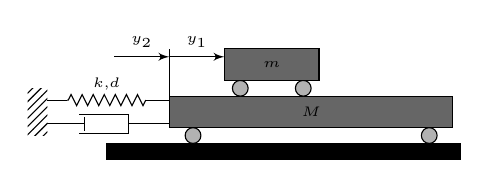
\begin{tikzpicture}[
        >=latex',
        spring/.style = {decorate,decoration={zigzag,amplitude=2pt,segment length=4pt}},
        damper/.style = {decorate,decoration={markings, mark connection node=dmp, mark=at position 0.5 with {
            \node (dmp) [thick,inner sep=0pt,transform shape,rotate=-90,minimum width=6pt,minimum height=15pt,draw=none] {};
            \draw ($(dmp.north east)+(2pt,0)$) -- (dmp.south east) -- (dmp.south west) -- ($(dmp.north west)+(2pt,0)$);
            \draw ($(dmp.north)+(0,-2.5pt)$) -- ($(dmp.north)+(0,2.5pt)$);
        }
        }}
    ]
    \draw[black, fill=black] (-0.5, 0) rectangle (4, 0.2);
    \draw[black, fill=black!30] (3.6,0.3) circle (0.1);
    \draw[black, fill=black!30] (0.6,0.3) circle (0.1);
    \draw[black, fill=black!60] (0.3, 0.4) rectangle (3.9, .8) node[pos=.5] {\tiny$M$};
    \draw[black, fill=black!30] (1.2, 0.9) circle (0.1);
    \draw[black, fill=black!30] (2,0.9) circle (0.1);
    \draw[black, fill=black!60] (1, 1) rectangle (2.2, 1.4) node[pos=.5] {\tiny$m$};
    \draw[black] (0.3,0.8) -- (0.3, 1.4);
    \draw[black] (0.3, 0.75) -- (0, 0.75);
    \draw[black] (0.3, 0.45) -- (0, 0.45);
    \draw[spring] (0,0.75) -- node[above] {\tiny$k$,$d$} +(-1,0);
    \draw[damper] (0,0.45) -- +(-1,0);
    \draw[black] (-1, 0.75) -- (-1.25, 0.75);
    \draw[black] (-1, 0.45) -- (-1.25, 0.45);
    \draw[fill,pattern=north east lines,draw=none,minimum width=0.75cm,minimum height=0.3cm,inner sep=0pt,outer sep=0pt] (-1.5, 0.3) rectangle
    (-1.25, 0.9);
    \draw[<-] (0.3, 1.3) -- node[above] {\tiny$y_2$} +(-0.7, 0);
    \draw[->] (0.3, 1.3) -- node[above] {\tiny$y_1$}(1,1.3);
\end{tikzpicture}

\end{document}
